\documentclass[10pt]{article}
\usepackage[T1]{fontenc} \usepackage{amsmath}
\usepackage{amsfonts}
\usepackage{amssymb}
\usepackage{listings}
\usepackage[version=4]{mhchem}
\usepackage{bbold}
\usepackage{graphicx}
\usepackage[export]{adjustbox}
\usepackage{xcolor}
\usepackage{bbold}
\usepackage{soul}
\usepackage{tikz,pgfplots, lipsum,lmodern}
\usepackage[T1]{fontenc}
\usepackage[ngerman]{babel}
\usepackage{adigraph}
\pgfplotsset{compat=1.18, width=10cm}
\usetikzlibrary{positioning}

\usepackage{nicematrix,tikz}
\usepackage[tmargin=2cm,rmargin=1in,lmargin=1in,margin=0.85in,bmargin=2cm,footskip=.2in]{geometry}
\usepackage{amsmath,amsfonts,amsthm,amssymb,mathtools}
\usepackage[varbb]{newpxmath}
\usepackage{xfrac}
\usepackage[makeroom]{cancel}
\usepackage{mathtools}
\usepackage{bookmark}
\usepackage{enumitem}
\usepackage[most,many,breakable]{tcolorbox}
\usepackage{varwidth}
\usepackage{varwidth}
\usepackage{etoolbox}
%\usepackage{authblk}
\usepackage{nameref}
\usepackage{multicol,array}
\usepackage{tikz-cd}
\usepackage[ruled,vlined,linesnumbered]{algorithm2e}
\usepackage{comment} % enables the use of multi-line comments (\ifx \fi) 
\usepackage{import}
\usepackage{xifthen}
\usepackage{pdfpages}

\definecolor{gre}{RGB}{101, 191, 127}
\definecolor{gree}{RGB}{7, 135, 44}

\newtcolorbox{defin}[2][]{colback=mygr!10,enhanced,title= #2,#1,
attach boxed title to top left={xshift=-4mm},boxrule=0pt,after skip=1cm,before skip=1cm,right skip=0cm,breakable,fonttitle=\bfseries,toprule=0pt,bottomrule=0pt,rightrule=0pt,leftrule=4pt,arc=0mm,skin=enhancedlast jigsaw,sharp corners,colframe=mygr,colbacktitle=mygr,boxed title style={
    frame code={ 
        \fill[mygr](frame.south west)--(frame.north west)--(frame.north east)--([xshift=3mm]frame.east)--(frame.south east)--cycle;
        \draw[line width=1mm,mygr]([xshift=2mm]frame.north east)--([xshift=5mm]frame.east)--([xshift=2mm]frame.south east);
        
        \draw[line width=1mm,mygr]([xshift=5mm]frame.north east)--([xshift=8mm]frame.east)--([xshift=5mm]frame.south east);
        \fill[mygr!40](frame.south west)--+(4mm,-2mm)--+(4mm,2mm)--cycle;
    }
}
}

\newtcolorbox{Box1}[2][]{sidebyside,
lower separated=false,
colback=white,
colframe=mygr,fonttitle=\bfseries,
colbacktitle=mygr,enhanced,
attach boxed title to top left={xshift=1cm,
yshift=-2mm},
title=#2,#1}

\newcommand{\uproman}[1]{\uppercase\expandafter{\romannumeral#1}}

\definecolor{mygr}{HTML}{2C3338}
\newcolumntype{?}[1]{!{\vrule width #1}}

\title{Report - Praxisblatt 1}
\author{Malte A. Weyrich & Jan P. Hummel}
\begin{document}

\maketitle
\section{Aufgabe}
\lipsum[1]
\begin{figure}[h]
    \centering
    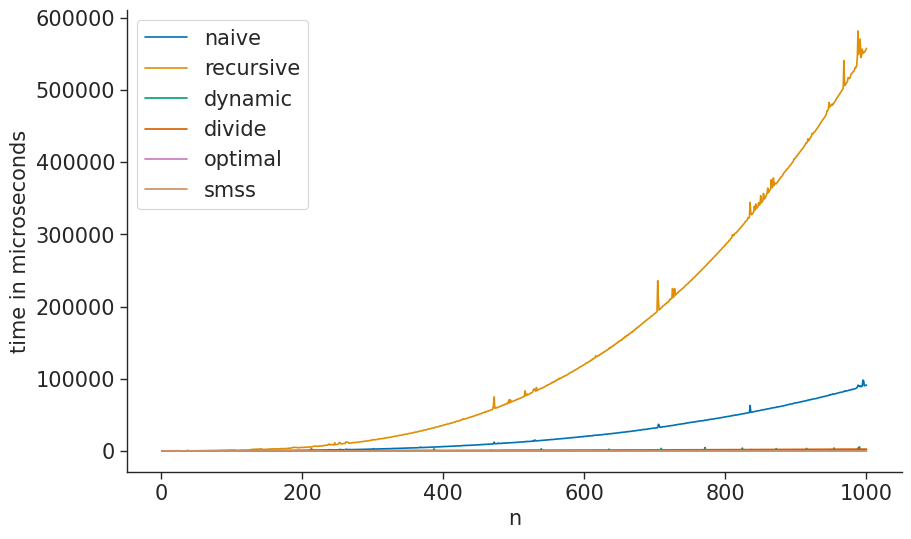
\includegraphics[width=0.8\textwidth]{../times_1000_all.png}
    \caption{all}
    \label{fig:Test}
\end{figure}

\section{Aufgabe}

\lipsum[1]
\subsection{2a - SMSS}\label{2a}
\lipsum[1]
\subsection{2b - SMSS mit minimaler Länge}\label{2b}
\lipsum[1]
\subsection{2c - Alle MSS} 

Für die 2c haben wir unseren ursprünglichen Ansatz nicht weiter verwendet. Der \textit{optimale Algorithmus} ist in sich selbst so effizient,
dass er null Folgen am Anfang und am Ende von Segmenten direkt ignoriert. Wir haben uns also überlegt, welcher der anderen 
Algorithmen mit eine möglichst guten Laufzeit, diese Fälle auch betrachtet. Wir haben uns dazu entschieden den \textit{dynamic programming Algorithmus} zu erweitern. Dieser hat nämlich den Vorteil
bereits ohne Erweiterungen, alle Kombinationen von Teilintervallen zu betrachten. Insbesondere die Teilintervalle,
die der \textit{optimale Algorithmus} nicht in Betracht zieht.

\textbf{Beispiel}

\begin{verbatim}
                              5 -5 9 -3 13 -5 5 -5 5
      optimal             :   -----+=====+----------

      tatsächliche MSS    :   -----+=====+----------
                              -----+==========+-----
                              -----+===============+
                              +==========+----------
                              +===============+-----
                              +====================+
\end{verbatim}

Der \textit{dynamic programming Algorithmus} betrachtet in dem oberen Beispiel alle der Teilfolgen. 
Also haben wir wieder wie in \ref{2a} eine äu\ss ere Liste mit inneren Listen erstellt, und für jeden neuen \textit{maxscore} eine neue innere Liste
erstellt, die dann mit allen gleichwertigen Segmenten (also allen Segmenten mit demselben \textit{maxscore}) befüllt wird, bis ein grö\ss erer \textit{maxscore} gefunden wird.
So findet der \textit{2\_c Algorithmus} also definitiv alle MSS, denn wir wissen bereits, dass der \textit{dynamic programming} Ansatz korrekt ist und
alle Kombinationen in Betracht zieht. Jedoch bu\ss t dieser Ansatz bei der Speicherkomplexität ein, das \textit{int[][]} Array wächst 
zu einem gegebenen Eingabe Vektor mit Länge $n$ exponentiell: $n^{2}$. D.h. für gro\ss e Eingaben verbrauchen wir enorm viel
Speicherplatz. 

Wie bereits in \textit{1. Theorie Blatt Aufgabe 2} gezeigt, benutzt der \textit{dynamic programming Algorithmus} immer nur 
die Hälfte des Arrays. Allgemein hat das Array die folgende Form:

$$
    \begin{pNiceMatrix}[left-margin]
    \times & \times & \times & \times & \times \\
           & \times & \times & \times & \times \\
           &        & \times & \times & \times \\ 
    \Block{2-2}<\Huge>{0}
           &        &        & \times & \times \\
           &        &        &        & \times \\
    \CodeAfter
     \tikz \draw (2-|1) -| (3-|2) -| (4-|3) -| (5-|4) -| (6-|5) ;
    \end{pNiceMatrix}
$$

Man könnte also Platz einsparen, wo nur \textit{0er} stehen:
\newpage

 \textbf{Beispiel}\\
 Betrachten wir die jeweiligen Endzustände der Datenstrukturen von Algorithmus \textit{2\_c} und der 
 speicherplatzoptimierten Variante \textit{2\_c\_1}:
 \begin{itemize}
     \item Eingabe: $v = \left\{5, -5, 9, -3, 13, -5, 5, -5, 5\right\}$
     \item Hardware: (\textit{Processor: AMD® Ryzen 7 pro 4750u with radeon graphics × 16; Memory: 16.0 GB})
 \end{itemize}

\begin{verbatim}
 Default Dynamic Programming (2_c) on v:
    0: [5 ,0 ,9 ,6 ,19,14,19,14,19]
    1: [0 ,-5,4 ,1 ,14,9 ,14,9 ,14]
    2: [0 ,0 ,9 ,6 ,19,14,19,14,19]
    3: [0 ,0 ,0 ,-3,10,5 ,10,5 ,10]
    4: [0 ,0 ,0 ,0 ,13,8 ,13,8 ,13]
    5: [0 ,0 ,0 ,0 ,0 ,-5,0 ,-5, 0]
    6: [0 ,0 ,0 ,0 ,0 ,0 ,5 , 0, 5]
    7: [0 ,0 ,0 ,0 ,0 ,0 ,0 ,-5,0 ]
    8: [0 ,0 ,0 ,0 ,0 ,0 ,0 ,0 ,5 ]
                               
 Max n on given Hardware: 30808:
 java -jar ... --algorithms 2_c --size 30808
\end{verbatim}

\begin{verbatim}
 Improved Dynamic Programming (2_c_1) on v:
    0: [5 ,0 ,9 ,6 ,19,14,19,14,19]
    1: [-5,4 ,1 ,14,9 ,14,9 ,14]
    2: [9 ,6 ,19,14,19,14,19]
    3: [-3,10,5 ,10,5 ,10]
    4: [13,8 ,13,8 ,13]
    5: [-5,0 ,-5,0]
    6: [5 ,0 ,5]
    7: [-5,0]
    8: [5]

 Max n on given Hardware: 44069:
 java -jar ... --algorithms 2_c_1 --size 44069
\end{verbatim}

Der \textit{improved dynamic programming 2\_c\_1} hat keine Position in der 
Datenstruktur, die ungenutzt bleibt. Der verbesserte Ansatz schafft es $13261$ zusätzliche
Zahlen zu verarbeiten, also ein $\approx 43\%$ grö\ss eres $n$ als der \textit{default 2\_c Algorithmus} 
(*auf der gegebenen Hardware).
\end{document}
